\documentclass{tufte-handout}
\setcounter{secnumdepth}{1}
\usepackage{amsmath}
\usepackage{natbib}
\newtheorem{app}{Application}
\newtheorem{example}{Example}
\newtheorem{exercise}{Exercise}
\newcommand{\define}{\textsc}
%\geometry{showframe}% for debugging purposes -- displays the margins
% all kinds of defaults from the template provided by overleaf
\usepackage{booktabs}
\usepackage{units}
\usepackage{fancyvrb}\fvset{fontsize=\normalsize}
\usepackage{multicol}
\usepackage{graphicx}
\usepackage{tikz}
\usetikzlibrary{patterns}
\setkeys{Gin}{width=\linewidth,totalheight=\textheight,keepaspectratio}
\graphicspath{{graphics/}}

% my own math shortcuts
\newcommand{\re}{\mathbb{R}}
\newcommand{\ve}{\mathcal{V}}

\title{Notes on stuff}
\author[Diego Navarro}
\date{}  


\begin{document}

\maketitle% this prints the handout title, author, and date

\begin{abstract}
\noindent This is a chatty introduction to simplicial complexes and related themes.  Please expect it to contain errors and leave me feedback whenever appropriate. 
\end{abstract}

%\printclassoptions
\section{Simplices in real spaces}

\subsection{The standard 1-simplex}
The standard 0-simplex $S_0$ is a real number $x_1\in[0,1]$.

The standard 1-simplex\marginnote{`Simplices' is the plural form of `simplex': one simplex, two simplices, three simplices.} $S_1$ is the set of pairs of positive real numbers $(x_1,x_2)$ such that $x_1+x_2=1$. If the pair $(x_1, x_2)$ is seen as an element of $\re^2$, this means the 1-simplex is the segment of the graph for $y=1-x$ where both $x,y$ are positive. A more verbose definition follows:
\begin{equation}
    S_1 := \{(x_1,x_2)\ |\ x_1+x_2=1, x_1>0, x_2>0\}
\label{standard-s1}
\end{equation}
\marginnote{My intuition for the 1-simplex is a ``budget'': the space of possible ways to allocate resources to two buckets}
More generally, the standard $n$-simplex is given by

\begin{equation}
    S_n := \left\{(x_1,\ldots,x_{n+1})\ |\ \sum_{i=1}^{n+1} x_i = 1, x_1,...,x_n >0 \right\}
\label{standard-sn}
\end{equation}
but I want to give some attention to $S_1$ first.
Note that from expression (\ref{standard-s1}) and the fact that $x_1,x_2$ are all positive, it follows that $x_1,x_2$ are each restricted to the unit interval $[0,1]$ Then we can equivalently define $S_1$ as
\begin{equation}
    S_1 = \bigcup_{\alpha\in [0,1]} \{{(x_1,\alpha)}\ |\ x_1 = 1-\alpha]\}
\label{union-1}
\end{equation}
This definition makes it clearer that, despite being originally identified as a pair of numbers in the unit interval, $S_1$ is actually tiny 1-dimensional subset of $[0,1]\times[0,1]$ which can be bijectively identified with the unit interval $[0,1]$. 

Note that the symmetry in $x_1+x_2=1$ means we could have swapped the order (or labels) of summands, taking unions over pairs like $(\alpha,x_2)$ would yield the same set. Visually we can imagine an animation that sweeps the vertical axis and records the points where $x=1-y$, or one that sweeps over the horizontal axis and records the points where $y=1-x$.\marginnote{This is overthinking for the 1-simplex but helps me see the 2- and especially the 3-simplex.
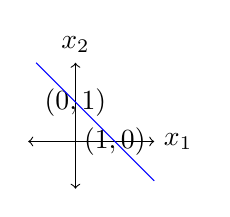
\begin{tikzpicture}
  \node (f) at (0,0.5) {$(0,1)$};
  \node (g) at (0.5,0) {$(1,0)$};
  \draw[<->] (-0.6, 0) -- (1, 0) node[right] {$x_1$};
  \draw[<->] (0, -0.6) -- (0, 1) node[above] {$x_2$};
  \draw[scale=0.5, domain=-1:2, smooth, variable=\x, blue] plot ({\x}, {1-\x});
\end{tikzpicture}

}

Note, finally, that the issue of length is more or less arbitrary: we could easily define scaled $1$-simplices corresponding to line segments of length $c>0$: 
{\[
c * S_n = \left\{(x_1,\dots,x_{n+1})\ \left| \sum_{i=1}^{n+1} x_i = c\right., x_i > 0 \text{ for each } i=1\dots n\right\}
\]

This is basically useful only to visualize the 2- and 3-simplex, so don't hang on to it too tightly.
}
\subsection{The standard 2-simplex}
The standard 2-simplex $S_2$ is the set of triples of positive real numbers $(x_1,x_2,x_3)$ such that $x_1+x_2+x_3=1$. Choosing the the third coordinate to range over, this means

\begin{equation}
    S_2 =  \bigcup_{\alpha\in[0,1]} \{(x_1,x_2,\alpha)\ |\ (x_1,x_2)\in (1-\alpha)*S_1\}
    \label{union-view-2}
\end{equation}
This is a union of line segments with lengths ranging from from an unit segment to a single point at $(0,0,1)$. We call the latter a \define{vertex}. Again, by trilateral symmetry $(1,0,0)$ and $(0,1,0)$ must also be vertices; and since we could have chosen to taken unions over pairs like $(x_1, \alpha,x_3)$ or $(\alpha,x_2,x_3)$, two additional unit segments must exist. If the 2-simplex is seen as embedded in $\re^3$, these must correspond to the line segments (\define{edges})
\begin{align*}
\{(x_1,1-x_1,0)\ &|\  x_1\in[0,1]\}\\
\{(0,x_2,1-x_2)\ &|\ x_2 \in[0,1]\}\\
\{(1-x_3,0,x_3)\ &|\ x_3\in[0,1]\}
\end{align*}

each of which is a 3D rotation of the 1-simplex $S_1$ to make the vertices touch. Again by trilateral symmetry, to each of these edges corresponds a range of shrinking segments filling the space until the next vertex. \marginnote{This is actually exploited in data visualization to represent objects that have three ingredients (like the NPK - nitrogen, phosphorus, potassium - composition of soils)}``Forgetting'' any one of these three coordinates (which is really predetermined by the rest), we project a triangle in one of the three planes that intersect at the origin. This triangle must be equilateral, since all edges are unit-length.
\subsection{Standard n-simplices revisited}
Generalizing the reasoning above, the standard $n$-simplex defined in expression (\ref{standard-sn}) can be rewritten as:


\begin{equation}
    S_n = \bigcup_{\alpha\in[0,1]} \{(x_1,\cdots,x_n,\alpha) | \ \{(x_1,\cdots,x_n)\in (1-\alpha)*S_{n-1}  \}
\label{union-sn}
\end{equation}
where $c*S_{n-1}$ is the set of $n$ positive reals that sum to $c$ (i.e. a ``scaled'' version of $S_{n-1}$).
\begin{exercise}
Show inductively that definitions (\ref{standard-sn}) and (\ref{union-sn}) are equivalent.
\end{exercise}
\begin{exercise}
What is $c*S_2$, geometrically? What does a $3$-simplex look like?
\end{exercise}
\subsection{General $n$-simplices}
For additional generality we can let simplices lie anywhere in real $n$-space as follows:

\begin{equation}
    S_{n}(u_1,\ldots,u_{n+1}) = \left\{\sum_{i=1}^{n+1} \theta_i u_i = 1\ |\  \theta_i>0; u_i\in \re^{n+1} \right\}
    \label{geometric-simplex}
\end{equation}

where $u_1,\ldots,u_{n+1}$ are linearly independent vectors. 

\begin{exercise}
Show that standard simplices are simplices in this more general sense. Hint: somehow rewrite the sum in (\ref{geometric-simplex}) in terms of vectors and matrices.
\end{exercise}
\begin{exercise}
Can the standard $S_n$ be recovered from any $S_n(u_1,\cdots,u_{n+1})$? How?
\end{exercise}

\section{Simplicial complexes}
\subsection{Abstract simplices}
\newcommand{\se}{\mathcal X}
\renewcommand{\sc}{\mathcal C}
Let $\ve$ be a finite set. The elements of $\ve$ are called \define{vertices}. An abstract $k$-simplex $\se$ is a subset of $\ve$ with $k+1$ elements. For example, $\ve$ is a set of people, 1-simplices can represent couples while 2-simplices represent three-person cliques. ($0$-simplices are one-element sets that we will also call vertices.)

Since $\ve$ is finite, its elements can be bijectively identified with the natural numbers $\{1,2,\cdots,\}$. For visual clarity when reading, we can further write a 1-simplex $\{1,2}\}$ as $[12]$, and generally a $k$-simplex $\{u,v,w,\ldots,z\}$ as $[uvw\ldots z]$ 

\begin{exercise}
What must $\ve$ be so that abstract simplices are simplices in real space?
\end{exercise}

A simplicial complex (SC)  is a set of abstract simplices $\sc=\{\se_1,\se_2,\ldots\}$ such that if a simplex $\se$ is in $\sc$, then all subsets of $\se$ are also in $\sc$.
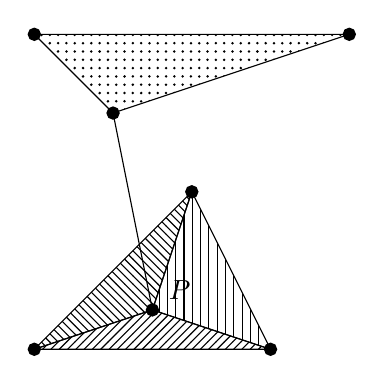
\begin{tikzpicture}
    \tikzstyle{point}=[circle,thick,draw=black,fill=black,inner sep=0pt,minimum width=4pt,minimum height=4pt]
    \node (a)[point] at (0,0) {};
    \node (b)[point] at (3,0) {};
    \node (c)[point] at (2,2) {};

    \begin{scope}[yshift=2cm]
    \node (d)[point] at (1,1) {};
    \node (e)[point] at (0,2) {};
    \node (f)[point] at (4,2) {};
    \end{scope}

    \node (p)[point,label={[label distance=0cm]5:$P$}] at (1.5,0.5) {};

    \draw[pattern=north east lines] (a.center) -- (p.center) -- (b.center) -- cycle;
    \draw[pattern=north west lines] (a.center) -- (p.center) -- (c.center) -- cycle;
    \draw[pattern=vertical lines]   (b.center) -- (p.center) -- (c.center) -- cycle;
    \draw[pattern=dots] (d.center) -- (e.center) -- (f.center) -- cycle;
    \draw (p.center) -- (d.center);
\end{tikzpicture}
\subsection{Graphs}
\newcommand{\maxdim}{\mathrm{max }\dim}
The following definition is not standard in classic treatments, but let $$\maxdim\ \sc := \max_{\se \in \sc} |\se|$$
(where $|X|$ is the number of elements in a finite set $X$).

A SC $\sc$ with $\maxdim \sc = 1$ is a \define{graph}.\marginnote{The whole goal of Section 1 was to build the intuition of how exactly simplices are $n$-dimensional triangles; however, we need to let go of the idea that these sets are embedded in a higher-dimensional ``space''. Instead, we're \emph{building} ``spaces'' by gluing simplices.} The idea is here is that if $[uv]$ is a line segment in $\sc$, then its ``endpoints'' $u$ and $v$ must also be in $\sc$ (due to how a SC is defined). 
\begin{exercise}
In the ordinary sense, a graph is a set $(\ve,\mathcal E)$ where $\mathcal E$ is a subset of $\ve\times \ve$ (a set of pairs of vertices). Are these definitions compatible?
\end{exercise}
\subsection{The clique complex}
Simplicial complexes may have elements with different dimensionality. A graph, for example, has elements with dimension 0 (vertices, which may or not be connected) and 1 (edges, in graph terminology). Note, in this vein, that the following SCs are different
\begin{align*}
    \sc_1 &= \{1,2,3,[12],[13],[23]\}\\
    \sc_2 &= \{1,2,3,[12],[13],[23],[123]\}
\end{align*}
despite being somewhat related: $\sc_1$ is a graph with three points and three edges that, if realized in $\re^2$ (by making each $1$-simplex the line segment that interpolates between its vertices) would suggest a triangular outlines -- while in contrast, $\sc_2$ has every element of $\sc_1$ in addition to the ``filled triangle'' $[123]$. 

This idea can be formalized (without handwaving invocations of geometric realizations) by the \textsc{clique complex}. In graph theory, a \textsc{clique} is a complete subgraph: a subset of a graph such that all of the vertices are connected. 

More exhaustively,  let  $\mathcal V$ be a set of vertices: its ``clique graph''\sidenote{More commonly called the ``complete'' graph} $(\mathcal V, \mathcal E)$ is obtained by attaching an edge set $\mathcal E$ containing all distinct pairs $\{u,v)\ | u\in \mathcal V, v \in \mathcal V, u\neq v\}$. A clique of a graph $(\mathcal G, \mathcal E)$ is simply a subgraph\sidenote{A subgraph is $(V',E'), V'\subset \mathcal V$ with  $E'\subset \mathcal E$} that is the clique graph of its vertices $V'$. 

While a clique graph is built from vertices, the clique complex is a SC built from a graph: besides the 0- (vertices) and 1-(simplices) present in the original graph, a higher-dimensional simplex is added for each clique. For example, if $\sc_1$ is seen as a graph, then  $\{[12],[23],[13]\}$ is a clique (all pairs of the vertices seen are present); therefore, we add the 2-simplex $[123]$. 


\section{Faces and cofaces}
The following set of simplices
\begin{align*}
    X_1 &= \{1,2,3,[123]\}\\
\end{align*}
is, by defintion, \textbf{not} a simplicial complex since $X_1 \ni [12]\subset [123]\not \in X_1$. That is,
if a SC has a ``triangle''', it must have its edges, and if it must have edges ($1$-simplices) at all it must have all of its vertices. This is the geometric intuition for the abstract definition of a SC:  whenever a $k$-simplex $\se$ is in a SC, its ``geometric boundaries'' (a set of $(k-1)$-simplices with $k+1$ elements) must also be in the SC. 

More thoroughly, a simplex is called a \define{face}\sidenote{
There seems to be some equivocation in the literature about this terminology. I'm following the usage in Schaub et al., but for Frohmader it seems that a ``face'' is \emph{any} subset of a simplex -- therefore $1,2,3$ would be faces of $[123]$; meanwhile, Schaub and I call a ``face'' would be, in his language, a ``facet''. Cf.  \cite{schaub2020random}

\cite{frohmader2008face}} 
\[
[12],[13],[23]
\]
are the three $1$-simplices that are faces of the $2$-simplex $[123]$
\begin{exercise}
Consider the set $\mathcal X$ that has one $k$-simplex, its faces, the faces of its faces and so on (the faces of vertices are all identically the empty set, so this is finite). Is this a SC? Is there a SC that has the $k$-simplex and fewer elements?
\end{exercise}

A dual concept is that of \define{cofaces}. Whereas faces are defined for simplices in isolation, a coface of a simplex $\se$ is a simplex $\se'$ that has $\se$ as a face. This implies an ambient universe of possible simplices where we can look for one with this property; simplicial complexes are the natural candidate, since the faces of any simplex $\se'\in \sc$ must also belong to $\sc$. 

For example, $[12]$ and $[13]$ are faces of $[123]$. This corresponds to the geometric intuition that these edges form the outlines of a $2$-simplex.
\begin{exercise}
Can the clique complex be defined in terms of cofaces?
\end{exercise}


\subsection{Adjacency}

It was briefly suggested that SCs were spaces built by gluing simplices. I will now try to make this a better-defined idea.

In some applications, graphs are defined as \define{incidence structures} on an edge set $\mathcal E$. What this means is that edges $[ij],[ik]$ are said to be ``incident'' (in some semantically meaningful fashion, such as pressure flow problems) whenever they share a vertex $i$. An incidence matrix $\mathcal I$ is, then, a linear transform $\mathcal E\to \ve$ that takes an edge to the vertices it connects.

Perhaps more commonly, graphs are also seen as \define{adjacency structures} on vertices. An adjacency matrix $\mathcal A$ is then a linear transform $\ve\to \ve$s which takes vertices to the vertices to which they're adjacent (or connected). 


In the general case for SCs, two simplices of $\sc$ are said to be \define{upper adjacent} if they have a common coface and \define{lower adjacent} if they have a common face. This is the precise way in which two vertices can be said to be (upper) adjacent in the ordinary graph (if they're faces of a common edge) sense, and two edges can be said to be lower adjacent (or incident) if they have a vertex in common.

In this way, we can arrange simplices (vertices, edges, triangles, tetrahedrons) in such a way that it makes sense that edges are joined at a vertex, or, maybe, tetrahedrons are joined by one point, edge or triangle. 
\section{Orientation}
\subsection{Orientation in graphs}
So far, every time I brought up graphs as an example of SCs, we've been implicitly using \emph{undirected graphs}, that is, graphs where the edge set can be exactly identified with a subset of $ve\times ve$. In applications, graphs are sometimes directed or even edge-weighted to represent directionality and quantitative flow. 

A directed (unweighted) graph can be defined as a pair $(\ve, \mathcal E)$ where $\mathcal E \subseteq \{-1,1\}\times V\times V$. This means that there can be two different edges between vertices $1,2$: one with negative sign, that we could identify with an \emph{ordering} of vertices like $(21)$ and another with a positive sign, identifiable with  $(12)$.
\subsection{Orientation in 2-simplices}
This becomes slightly more confusing in the case of 2-simplices (``triangles'') too: an arbitrary $\se=[ijk]$ has $3!$ possible orderings
\begin{align*}
(ijk),(ikj),(kij),(kji),(jik),(jki).
\end{align}

but there are reasons to understand $(ijk)$ and $(kij)$ to have the same \define{orientation}. Imagine a walker that follows $(ijk)$ from vertex to vertex endlessly: its path will be the sequence $ijkijkijk\ldots$. Notice that the entire corresponding path for $(kji)$ is contained in the path for $(ijk)$  there. Meanwhile, $(ijk)$ and $(jik)$ are different: they point to opposite directions along the loop. 



Alternatively: if you actually draw a triangle, label its vertices $i,j,k$ and place arrows $i\to j\to k$, the same will become clear.
\section{Chain complexes}
A vector \define{chain complex}\sidenote{}
is a pair
\[
\left(\{V_i\ | i\in\mathbb Z\}, \right \{\phi_i\colon V_i \to V_{i-1}\ |\ i \in \mathbb Z\})
\]
where $V_i$ are vector spaces and $\phi_i \circ \phi_{i+1} = 0$ (the constant zero map $x \mapsto 0$), i.e.
\[
\cdots \xrightarrow{\phi_2} V_2 \xrightarrow{\phi_1} V_1\xrightarrow{\phi_0} V_0 \xrightarrow{\phi_{-1}} \cdots 
\]

In topology, the maps $\phi_i$ often have the interpretation of boundary operators, in which case they're also commonly written as $\partial_i$.

\nocite{*}
\bibliography{refs}
\bibliographystyle{siam}



\end{document}
